\chapter{Methods}
\label{sec:chap4}
We begin this chapter introducing the data used for our experiments as well as some additional sources for further research. We continue by briefly discussing the methods of converting 3D meshes to various other representations and we end with discussing our software decisions.

\section{Datasets}
In this section we introduce datasets of 3D models which we used or considered to use for testing.

\subsection{ModelNet40}
ModelNet \cite{wu_3d_2014} is one of the most well-known and commonly used dataset containing annotated 3D models in a mesh format. It was developed by a team at Princeton University. Its subset, called ModelNet40, in particular is used as a baseline for testing different approaches. We therefore decided to use this dataset as a starting point for our evaluations. ModelNet40 contains forty different categories and 12 311 individual models. The dataset has an official split to training and testing subsets, which we adhere to in all cases. The test set contains 2648 models and is never used for training. \par
The models in original ModelNet40 are not aligned and have widely different scales. Therefore when preprocessing the data for neural networks we rescale all models to fit a  unit sphere and we use manually aligned version of the dataset \cite{sedaghat_orientation-boosted_2016}. Also the categories are not equally populated for example there are over 700 airplane models and only over 100 wardrobe models. The exact numbers of models in particular categories can be found in \hyperref[Table:modelnetcats]{Table 4.1}. ModelNet40 contains files in .off format so our scripts have to be able to read this particular format. The dataset is available to download for academic purposes.

\begin{table}[]
	\centering
	\begin{tabular}[t]{lccl}
		\hline
		\textbf{Category} & \textbf{Train} & \textbf{Test} & \hspace{4pt} \\ \hline
		airplane          & 626            & 100           &                \\
		bathtub           & 106            & 50            &                \\
		bed               & 515            & 100           &                \\
		bench             & 173            & 20            &                \\
		bookshelf         & 572            & 100           &                \\
		bottle            & 335            & 100           &                \\
		bowl              & 64             & 20            &                \\
		car               & 197            & 100           &                \\
		chair             & 889            & 100           &                \\
		cone              & 167            & 20            &                \\
		cup               & 79             & 20            &                \\
		curtain           & 138            & 20            &                \\
		desk              & 200            & 86            &                \\
		door              & 109            & 20            &                \\
		dresser           & 200            & 86            &                \\
		flower pot        & 149            & 20            &                \\
		glass box         & 171            & 100           &                \\
		guitar            & 155            & 100           &                \\
		keyboard          & 145            & 20            &                \\
		lamp              & 124            & 20            &                \\
		                  &                &               &                \\ \hline
		                  &                &
	\end{tabular}
     \bigskip
	\begin{tabular}[t]{llcc}
		\hline
		\hspace{4pt} & \textbf{Category} & \textbf{Train} & \textbf{Test} \\ \hline
		             & laptop            & 149            & 20            \\
		             & mantel            & 284            & 100           \\
		             & monitor           & 465            & 100           \\
		             & night stand       & 200            & 86            \\
		             & person            & 88             & 20            \\
		             & piano             & 231            & 100           \\
		             & plant             & 240            & 100           \\
		             & radio             & 104            & 20            \\
		             & range hood        & 115            & 100           \\
		             & sink              & 128            & 20            \\
		             & sofa              & 680            & 100           \\
		             & stairs            & 124            & 20            \\
		             & stool             & 90             & 20            \\
		             & table             & 392            & 100           \\
		             & tent              & 163            & 20            \\
		             & toilet            & 344            & 100           \\
		             & tv stand          & 267            & 100           \\
		             & vase              & 475            & 100           \\
		             & wardrobe          & 87             & 20            \\
		             & xbox              & 103            & 20            \\
		             & \textbf{Total}    & \textbf{9843 } & \textbf{2468} \\ \hline

	\end{tabular}
	
	\caption{List of ModelNet40 categories and the number of training and test models in each category.}
	\label{Table:modelnetcats}
\end{table}

\subsection{ShapeNetCore}
ShapeNet \cite{chang_shapenet:_2015} is an ongoing effort to establish a richly-annotated, large-scale dataset of 3D shapes. ShapeNet is a collaborative effort between researchers at Princeton, Stanford and Toyota Technological Institute at Chicago. We used its subset called ShapeNetCore which contains 51 209 individual models in 55 categories. There is also an official split to training, test and validation sets. However, this split does not contain all models and is not divided uniformly. We therefore decided to construct our own split -- 80\% of models in each category is assigned to training set and the rest to test sest. By doing this we obtained a training set with 40 939 models and test set with 10 270 models. \par \hyperref[Table:shapenetcats]{Table 4.2} lists the exact numbers of models in particular categories. During our exploration of the dataset we noticed that some models are assigned to more than one category so we were forced to choose one of them somewhat arbitrarily. You can find our final split into sets and categories in csv file [priloha x].  \par
All models in ShapeNetCore are already aligned and rescaled to fit a unit sphere. The categories are not distributed equally at all as you can see from the table. The dataset is also freely available to download for academic purposes.


\begin{table}[]
	\centering
	\begin{tabular}[t]{lccl}
		\hline
		\textbf{Category}  & \textbf{Train} & \textbf{Test} & \hspace{4pt} \\ \hline
		airplane           & 3235           & 810           &              \\
		ashcan             & 275            & 68            &              \\
		bag                & 66             & 17            &              \\
		basket             & 82             & 21            &              \\
		bathtub            & 684            & 172           &              \\
		bed                & 184            & 49            &              \\
		bench              & 1451           & 362           &              \\
		birdhouse          & 58             & 15            &              \\
		bookshelf          & 362            & 90            &              \\
		bottle             & 395            & 102           &              \\
		bowl               & 146            & 39            &              \\
		bus                & 751            & 188           &              \\
		cabinet            & 1247           & 315           &              \\
		camera             & 90             & 23            &              \\
		can                & 84             & 21            &              \\
		cap                & 44             & 12            &              \\
		car                & 2811           & 703           &              \\
		cellular telephone & 665            & 166           &              \\
		chair              & 5391           & 1354          &              \\
		clock              & 521            & 130           &              \\
		computer keyboard  & 51             & 13            &              \\
		dishwasher         & 74             & 19            &              \\
		display            & 874            & 218           &              \\
		earphone           & 58             & 15            &              \\
		faucet             & 593            & 149           &              \\
		file               & 230            & 59            &              \\
		guitar             & 637            & 160           &              \\
		helmet             & 129            & 33            &              \\ \hline
		                   &                &
	\end{tabular}
	\begin{tabular}[t]{llcc}
		\hline
		\hspace{4pt} & \textbf{Category} & \textbf{Train} & \textbf{Test}  \\ \hline
		             & jar               & 466            & 114            \\
		             & knife             & 339            & 85             \\
		             & lamp              & 1853           & 464            \\
		             & laptop            & 360            & 91             \\
		             & loudspeaker       & 1274           & 319            \\
		             & mailbox           & 74             & 19             \\
		             & microphone        & 53             & 14             \\
		             & microwave         & 122            & 30             \\
		             & motorcycle        & 269            & 68             \\
		             & mug               & 171            & 43             \\
		             & piano             & 191            & 48             \\
		             & pillow            & 76             & 20             \\
		             & pistol            & 247            & 60             \\
		             & pot               & 439            & 110            \\
		             & printer           & 132            & 33             \\
		             & remote control    & 52             & 14             \\
		             & rifle             & 1864           & 467            \\
		             & rocket            & 68             & 17             \\
		             & skateboard        & 121            & 31             \\
		             & sofa              & 2406           & 603            \\
		             & stove             & 174            & 44             \\
		             & table             & 6702           & 1676           \\
		             & telephone         & 206            & 52             \\
		             & tower             & 98             & 25             \\
		             & train             & 311            & 78             \\
		             & vessel            & 1550           & 388            \\
		             & washer            & 133            & 34             \\
		             & \textbf{Total}    & \textbf{40939} & \textbf{10270} \\ \hline
	\end{tabular}
	
	
	\caption{List of ShapeNetCore categories and their counts.}
	\label{Table:shapenetcats}
\end{table}

\subsection{Other 3D Datasets}
In this section we mention several publicly available datasets containing 3D models which can be used for further research. \par
Both ModelNet and ShapeNet contain much more models than the standardized subsets we used for our evaluation. Therefore there is an option to download the whole datasets or to construct custom subsets. \par
A Large Dataset of Object Scans \cite{choi_large_2016} is a dataset concentrating on video scan to 3D model reconstruction but we suppose it can be used for learning classification as well. 
ObjectNet3D \cite{xiang_objectnet3d:_2016} focuses on image to 3D model reconstruction and therefore contains a large number of 3D models that can be used for classification training.
SUNCG dataset \cite{song_semantic_2017} contains entire indoor scenes but is annotated on the level of single objects and therefore can be parsed and used for classification. 
SceneNN \cite{hua_scenenn:_2016} dataset contains a large number of scenes which are richly annotated and can be split into single objects similarly to the previous dataset.

\section{Data Conversion}
As mentioned in previous chapters,  mesh files, in which most existing 3D models are saved, are not suitable for direct processing by neural networks. Therefore we have to be able to convert meshes to voxels, images or point clouds.

\subsection{Mesh to Voxels}
In order to use voxel based systems we need to convert mesh files to voxel occupancy grids. For this purpose we have chosen the OpenVDB library, which is free, open-source and offers python scripting \cite{museth_openvdb:_2013}. OpenVDB offers voxelization as one of its core functions, implemented in C++. We supply python scripts for voxelization of ModelNet40 and ShapeNetCore datasets using python multiprocessing to parallelize the computation. (ref the the user guide that describes how to use the scripts?) Still it can take several hours to process the whole dataset as we need to voxelize multiple rotations for each model. 

\begin{figure}[!h]
	\centering
	\subfloat[Original voxel representation provided by authors of VRN]{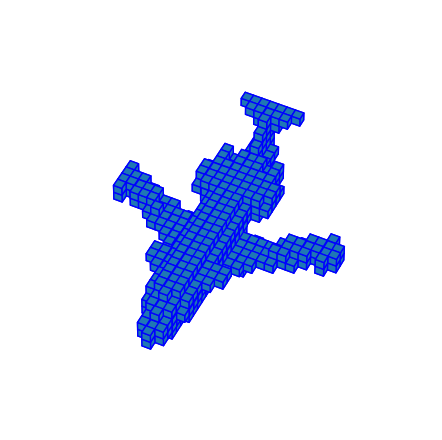
\includegraphics[width=0.44\columnwidth]{./img/myplane_2}}
	\qquad
	\subfloat[Our voxelization using OpenVDB]{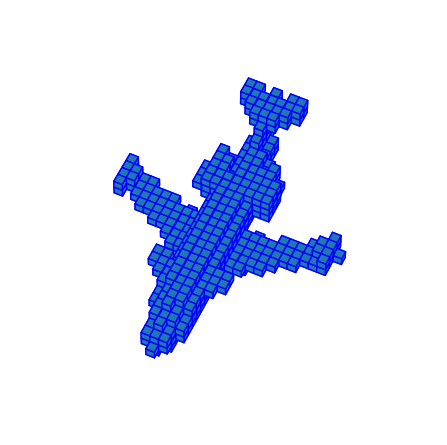
\includegraphics[width=0.44\columnwidth]{./img/vrnesn_plane_2}}
	\caption{Illustration of voxel representation}
\end{figure}

\subsection{Mesh to Images}
For multi-view based neural network we have to be able to render images taken from arbitrary viewpoints of a 3D mesh. Firstly we tried to replicate results used by the authors of RotationNet \cite{kanezaki_rotationnet:_2016} and we used pbrt \cite{pharr_physically_2010}, which is physically based rendering software with publicly available code. This turned out to be a plausible approach. 
Later in our research we found blender scripts from the authors of MVCNN2 \cite{su_deeper_2018}. These work faster and achieve better accuracy than both ours and original RotationNet images. In our framework we provide both approaches implemented with python scripts and multiprocessing support. 

\begin{figure}[!h]
	\centering
	\subfloat[Original rendering provided by authors of Rotation Net]{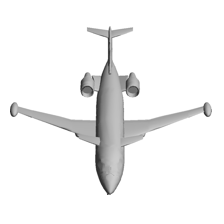
\includegraphics[width=0.44\columnwidth]{./img/airplane_rotnet}}
	\qquad
	\subfloat[Our pbrt rendering]{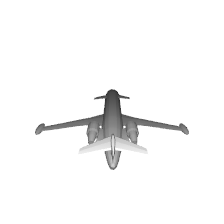
\includegraphics[width=0.44\columnwidth]{./img/airplane_pbrt}}

	\centering
	\subfloat[Depth image provided by authors of MVCNN2]{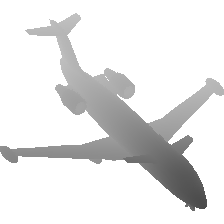
\includegraphics[width=0.44\columnwidth]{./img/airplane_depth}}
	\qquad
	\subfloat[Shaded image provided by authors of MVCNN2]{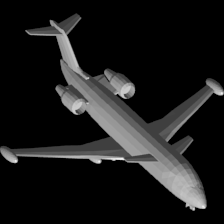
\includegraphics[width=0.44\columnwidth]{./img/airplane_shaded}}
	\caption{Illustration of different image representations}
\end{figure}

\subsection{Mesh to Point Cloud}
For the use of point cloud based neural networks we have to be able to construct a point cloud from a 3D mesh. This is a much more straightforward problem than the conversions described above. A point cloud is created by random sampling from the polygons forming the mesh. Firstly, we select a polygon with a probability proportional to the area of that polygon. Than we sample a random point within the selected polygon by generating random barycentric coordinates. We provide a python script with support for multiprocessing and this is sufficiently fast for our purposes.  

\begin{figure}[!h]
	\centering
	\subfloat[Original point cloud representation provided by authors of PointNet]{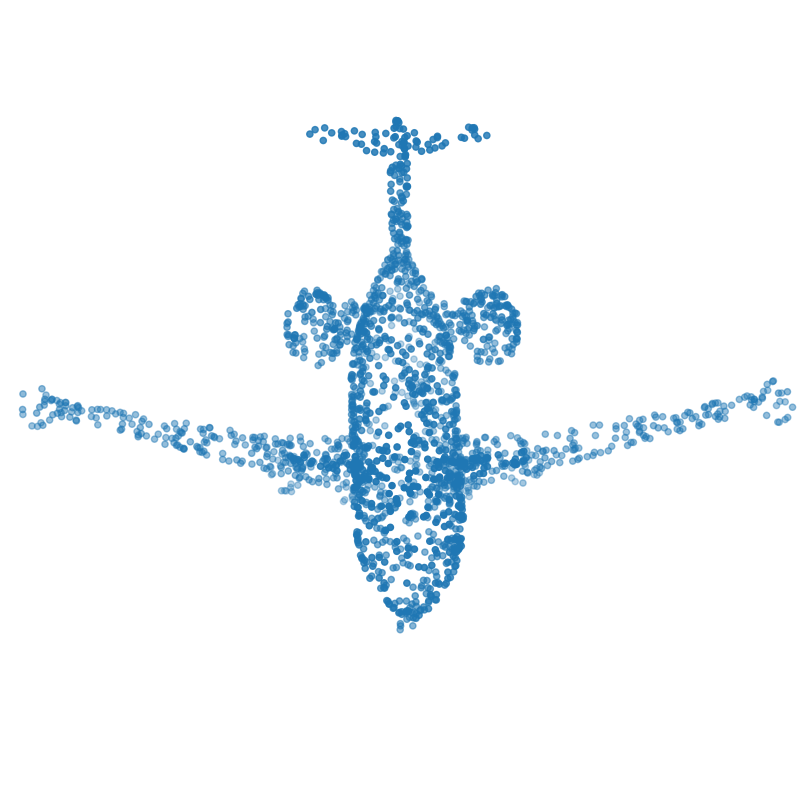
\includegraphics[width=0.44\columnwidth]{./img/myplane_1}}
	\qquad
	\subfloat[Our point cloud representation]{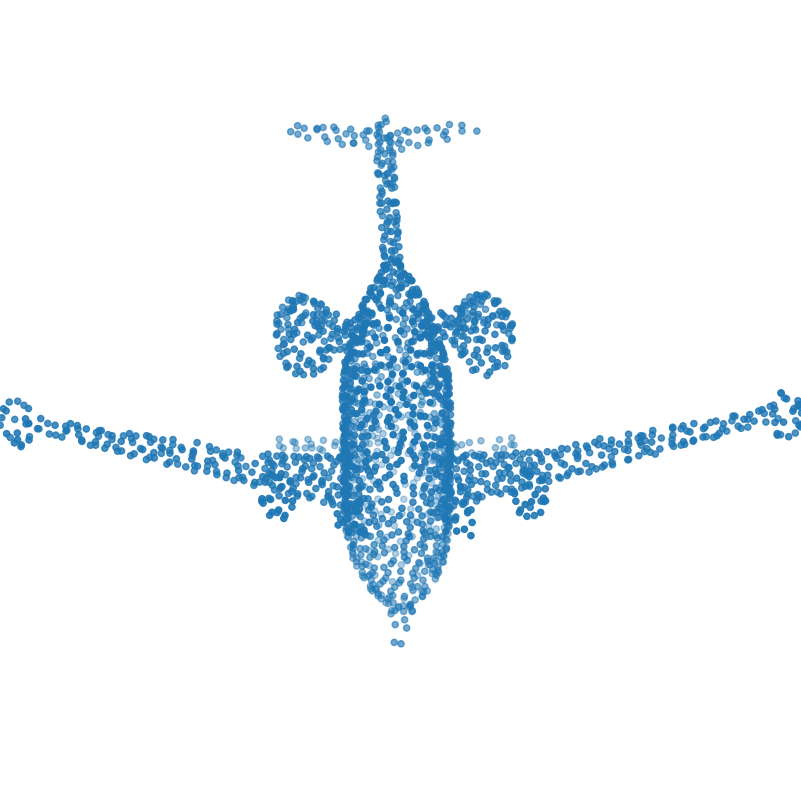
\includegraphics[width=0.44\columnwidth]{./img/pnet_plane_1}}
	\caption{Illustration of point cloud representation}
\end{figure}

\section{Technical Setup}
This section provides a brief summary of software choices we made. For information about prerequisites and structure of our framework, please consult the manual [příloha]. \par
As one of our main goals is to provide the academical community with easily runnable code, we opted for a solution using Docker \cite{merkel_docker:_2014}. Docker is a program used to run software packages called containers. Containers are isolated bundles of software, libraries and configurations. The specification of a container is called an image. An image contains a so called Dockerfile which defines the image, allowing automatic installation of all dependencies, setting up configurations, etc. Every neural network and data conversion package is thus a completely independent piece of software which can be run almost without any prerequisites. We consider this to be one of the main contributions of our work. \par
As all the machine learning frameworks we encountered support handling by python scripts and python is the most commonly used programming language in machine learning and artificial intelligence, we naturally use it for most of our code. We also preferred libraries for data conversion which support python. Some of the neural networks are implemented in such a way that they accept a purely pythonic file format as their input. So library not supporting python would require one more data conversion step.\par
We currently support only Linux, but Docker can be run on Windows as well and we believe that our framework can be extended to run on Windows without great difficulties. 
